%%%%%%%%%%%%%%%%%%%%%%%%%%%%%%%%%%%%%%%%%
% fphw Assignment
% LaTeX Template
% Version 1.0 (27/04/2019)
%
% This template originates from:
% https://www.LaTeXTemplates.com
%
% Authors:
% Class by Felipe Portales-Oliva (f.portales.oliva@gmail.com) with template 
% content and modifications by Vel (vel@LaTeXTemplates.com)
%
% Template (this file) License:
% CC BY-NC-SA 3.0 (http://creativecommons.org/licenses/by-nc-sa/3.0/)
%
%%%%%%%%%%%%%%%%%%%%%%%%%%%%%%%%%%%%%%%%%

%----------------------------------------------------------------------------------------
%	PACKAGES AND OTHER DOCUMENT CONFIGURATIONS
%----------------------------------------------------------------------------------------

\documentclass[
	12pt, % Default font size, values between 10pt-12pt are allowed
	%letterpaper, % Uncomment for US letter paper size
	%spanish, % Uncomment for Spanish
	german, % Uncomment for German
]{fphw}

% Template-specific packages

%encoding
%--------------------------------------
\usepackage[utf8]{inputenc}
\usepackage[T1]{fontenc}
%--------------------------------------
 
%German-specific commands
%--------------------------------------
\usepackage[ngerman]{babel}
\usepackage{csquotes}

\usepackage{mathpazo} % Use the Palatino font

\usepackage{graphicx} % Required for including images

\usepackage{booktabs} % Required for better horizontal rules in tables

\usepackage{float} % Floating figures

\usepackage{listings} % Required for insertion of code

\usepackage{enumerate} % To modify the enumerate environment

\usepackage{amsmath} % Math

%----------------------------------------------------------------------------------------
%	ASSIGNMENT INFORMATION
%----------------------------------------------------------------------------------------

\title{Algorithmisch lösbare und algorithmisch unlösbare Probleme} % Assignment title

\author{Alexandra Maximova} % Student name

\date{22.04.2020} % Due date

\institute{ETH Zurich \\ Lehrdiplom Informatik} % Institute or school name

\class{Fachdidaktik 2 (Berechenbarkeit)} % Course or class name

\professor{Giovanni Serafini, Juraj Hromkovič} % Professor or teacher in charge of the assignment

%----------------------------------------------------------------------------------------

\begin{document}

\maketitle % Output the assignment title, created automatically using the information in the custom commands above

%----------------------------------------------------------------------------------------
%	ASSIGNMENT CONTENT
%----------------------------------------------------------------------------------------

\section*{Aufgabe zur Reduktion im 'positiven' Sinne}

\begin{problem}
	Nehmen wir an, wir haben einen Algorithmus B, um den Logarithmus einer beliebigen Zahl \(x \geq 0\) zur Basis \(b\) zu berechnen, d.h. \(log_b(x)\). Entwickle mittels Reduktion einen Algorithmus zur Berechnung vom Logarithmus zur Basis \(a\).
	
	Heute scheint uns dieses Problem künstlich und konstruiert zu sein, aber vor nicht all zu langer Zeit war das tatsächlich praxisrelevant. Bevor die modernen Taschenrechner erschienen, die Logarithmen in jeder Basis berechnen können, haben Ingenieure täglich mit Tabellen gearbeitet, die die Logarithmen zur Basis \(10\) für sehr viele Zahlen aufgelistet haben. Manchmal brauchten sie den Logarithmus zu einer anderen Basis, die nicht tabelliert war; das konnten sie aber einfach aus den Werten der Tabelle berechnen.
	
	Zur Erinnerung, der Logarithmus ist bijektiv für \(x \geq 0\) und es gelten folgende Rechenregeln:
	\begin{enumerate}[(a)]
		\item \( log(x \cdot y) = log(x) + log(y) \)
		\item \( log(x^y) = y \cdot log(x) \)
	\end{enumerate}
\end{problem}


%------------------------------------------------

\subsection*{Musterlösung}

Bezeichnen wir durch \(U_B\) das Problem, den Logarithmus zur Basis \(b\) zu berechnen und durch \(U_A\) das Problem, den Logarithmus zur Basis \(a\) zu berechnen. Wir werden \(U_A \leq_{Alg} U_B\) zeigen, d.h. \(U_A\) auf \(U_B\) reduzieren. Dafür müssen wir und einen Algorithmus \(A\) konstruieren, welcher den gegebenen Algorithmus \(B\) benutzt und den Logarithmus zur Basis \(a\) berechnet.

Wir möchten also \(log_a(x)\) berechnen und können dafür den Logarithmus zur Basis \(b\) von beliebigen Zahlen mit dem Algorithmus \(B\) berechnen. Sei \(y = log_a(x)\). Dann, aus der Definition des Logarithmus, muss \(a^y = x\) sein. Da nach Annahme \(x \geq 0 \), können wir auf beiden Seiten der Gleichung die bijektive Funktion \(log_b\) anwenden, ohne dass sich die Menge der Resultate ändert.
\begin{alignat*}{3}
a^y &= x & \\
log_b(a^y) &= log_b(x) & \\
y \cdot log_b(a) &= log_b(x) & \quad \text{(Rechenregeln anwenden)} \\
log_a(x) \cdot \log_b(a) &= log_b(x) & \quad \text{(Definition für \(y\) einsetzen)}\\
log_a(x) &= \frac{log_b(x)}{log_b(a)} & \quad \text{(\(a \neq 1\))}\\
\end{alignat*}
Im letzten Schritt haben wir beide Seiten der Gleichung durch \(log_b(a)\) geteilt. Das können wir genau dann machen, wenn \(a \neq 1\). Das können wir hier annehmen, weil es keinen Sinn hat, \(1\) als die Basis eines Logarithmus zu verwenden.

Den Algorithmus \(A\) konstruieren wir folgendermassen: Wir benutzen den Algorithmus \(B\), um \(log_b(x)\) und \(log_b(a)\) zu berechnen, und dann ermitteln wir die Antwort, indem wir diese zwei Zahlen durcheinander teilen.

\begin{figure}[H]
	\centering
	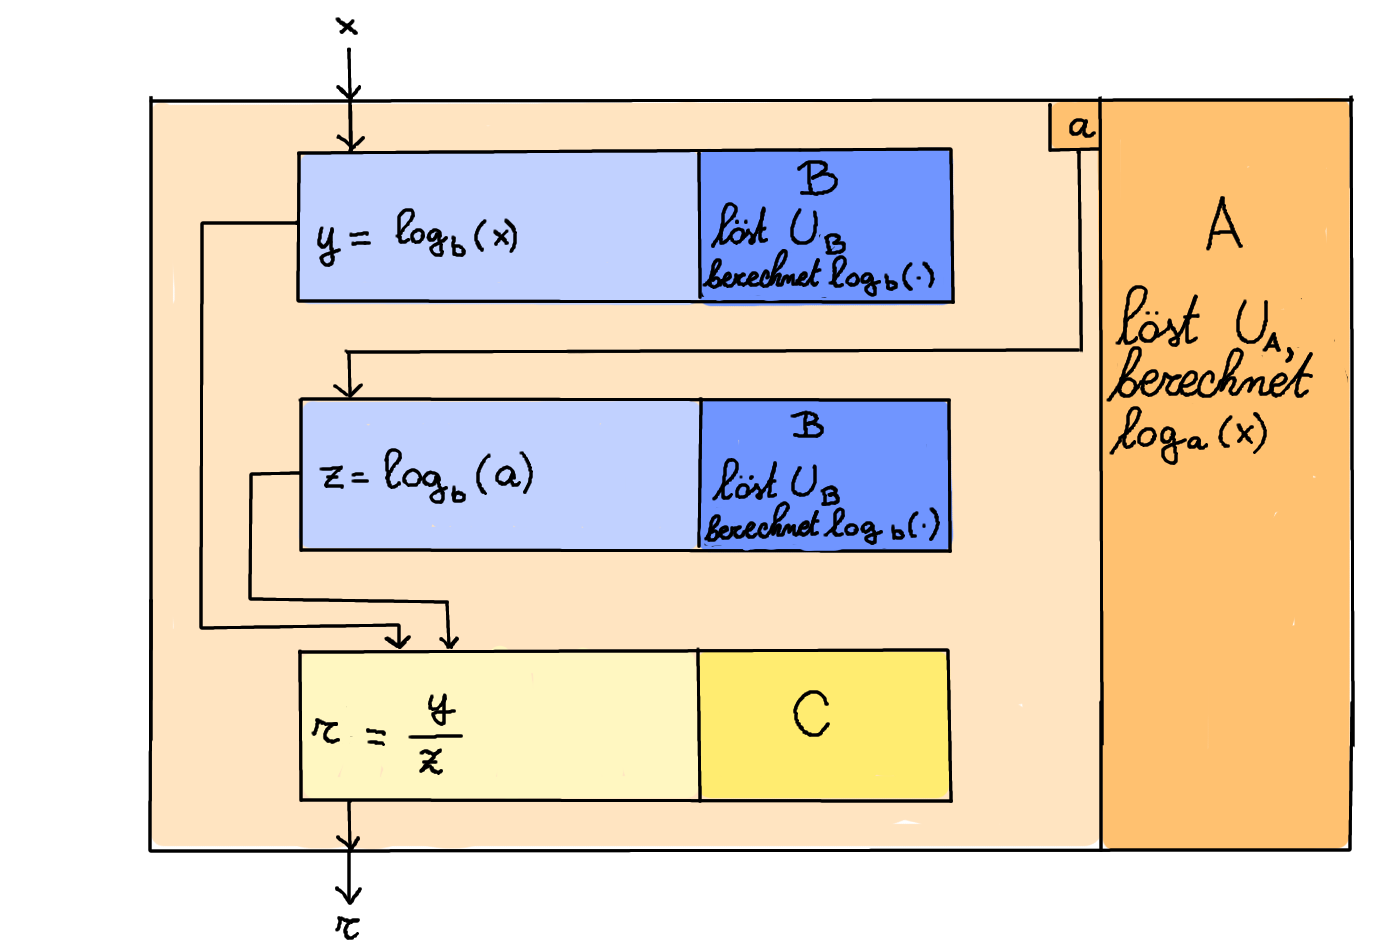
\includegraphics[width=\textwidth]{Positiv.png}
	\caption{Reduktion von \(U_A\) auf \(U_B\).}
\end{figure}

%----------------------------------------------------------------------------------------

\section*{Aufgabe zur Reduktion im 'negativen' Sinne}

\begin{problem}
Wir haben alle schon mal von der Quadratur des Kreises gehört und dass es unmöglich sein soll. Genauer, das Problem \(Q_{\bigcirc}\) besteht darin, mit Zirkel und Lineal in endlich vielen Schritten aus einem gegebenem Kreis ein Quadrat mit gleichem Flächeninhalt zu konstruieren. Der Beweis, dass es keinen ZL-Algorithmus (Zirkel-Lineal Algorithmus) für \(Q_{\bigcirc}\) gibt, ist nicht trivial und wir glauben an dieser Stelle den Mathematikern, die es bewiesen haben.

\begin{figure}[H]
	\centering
	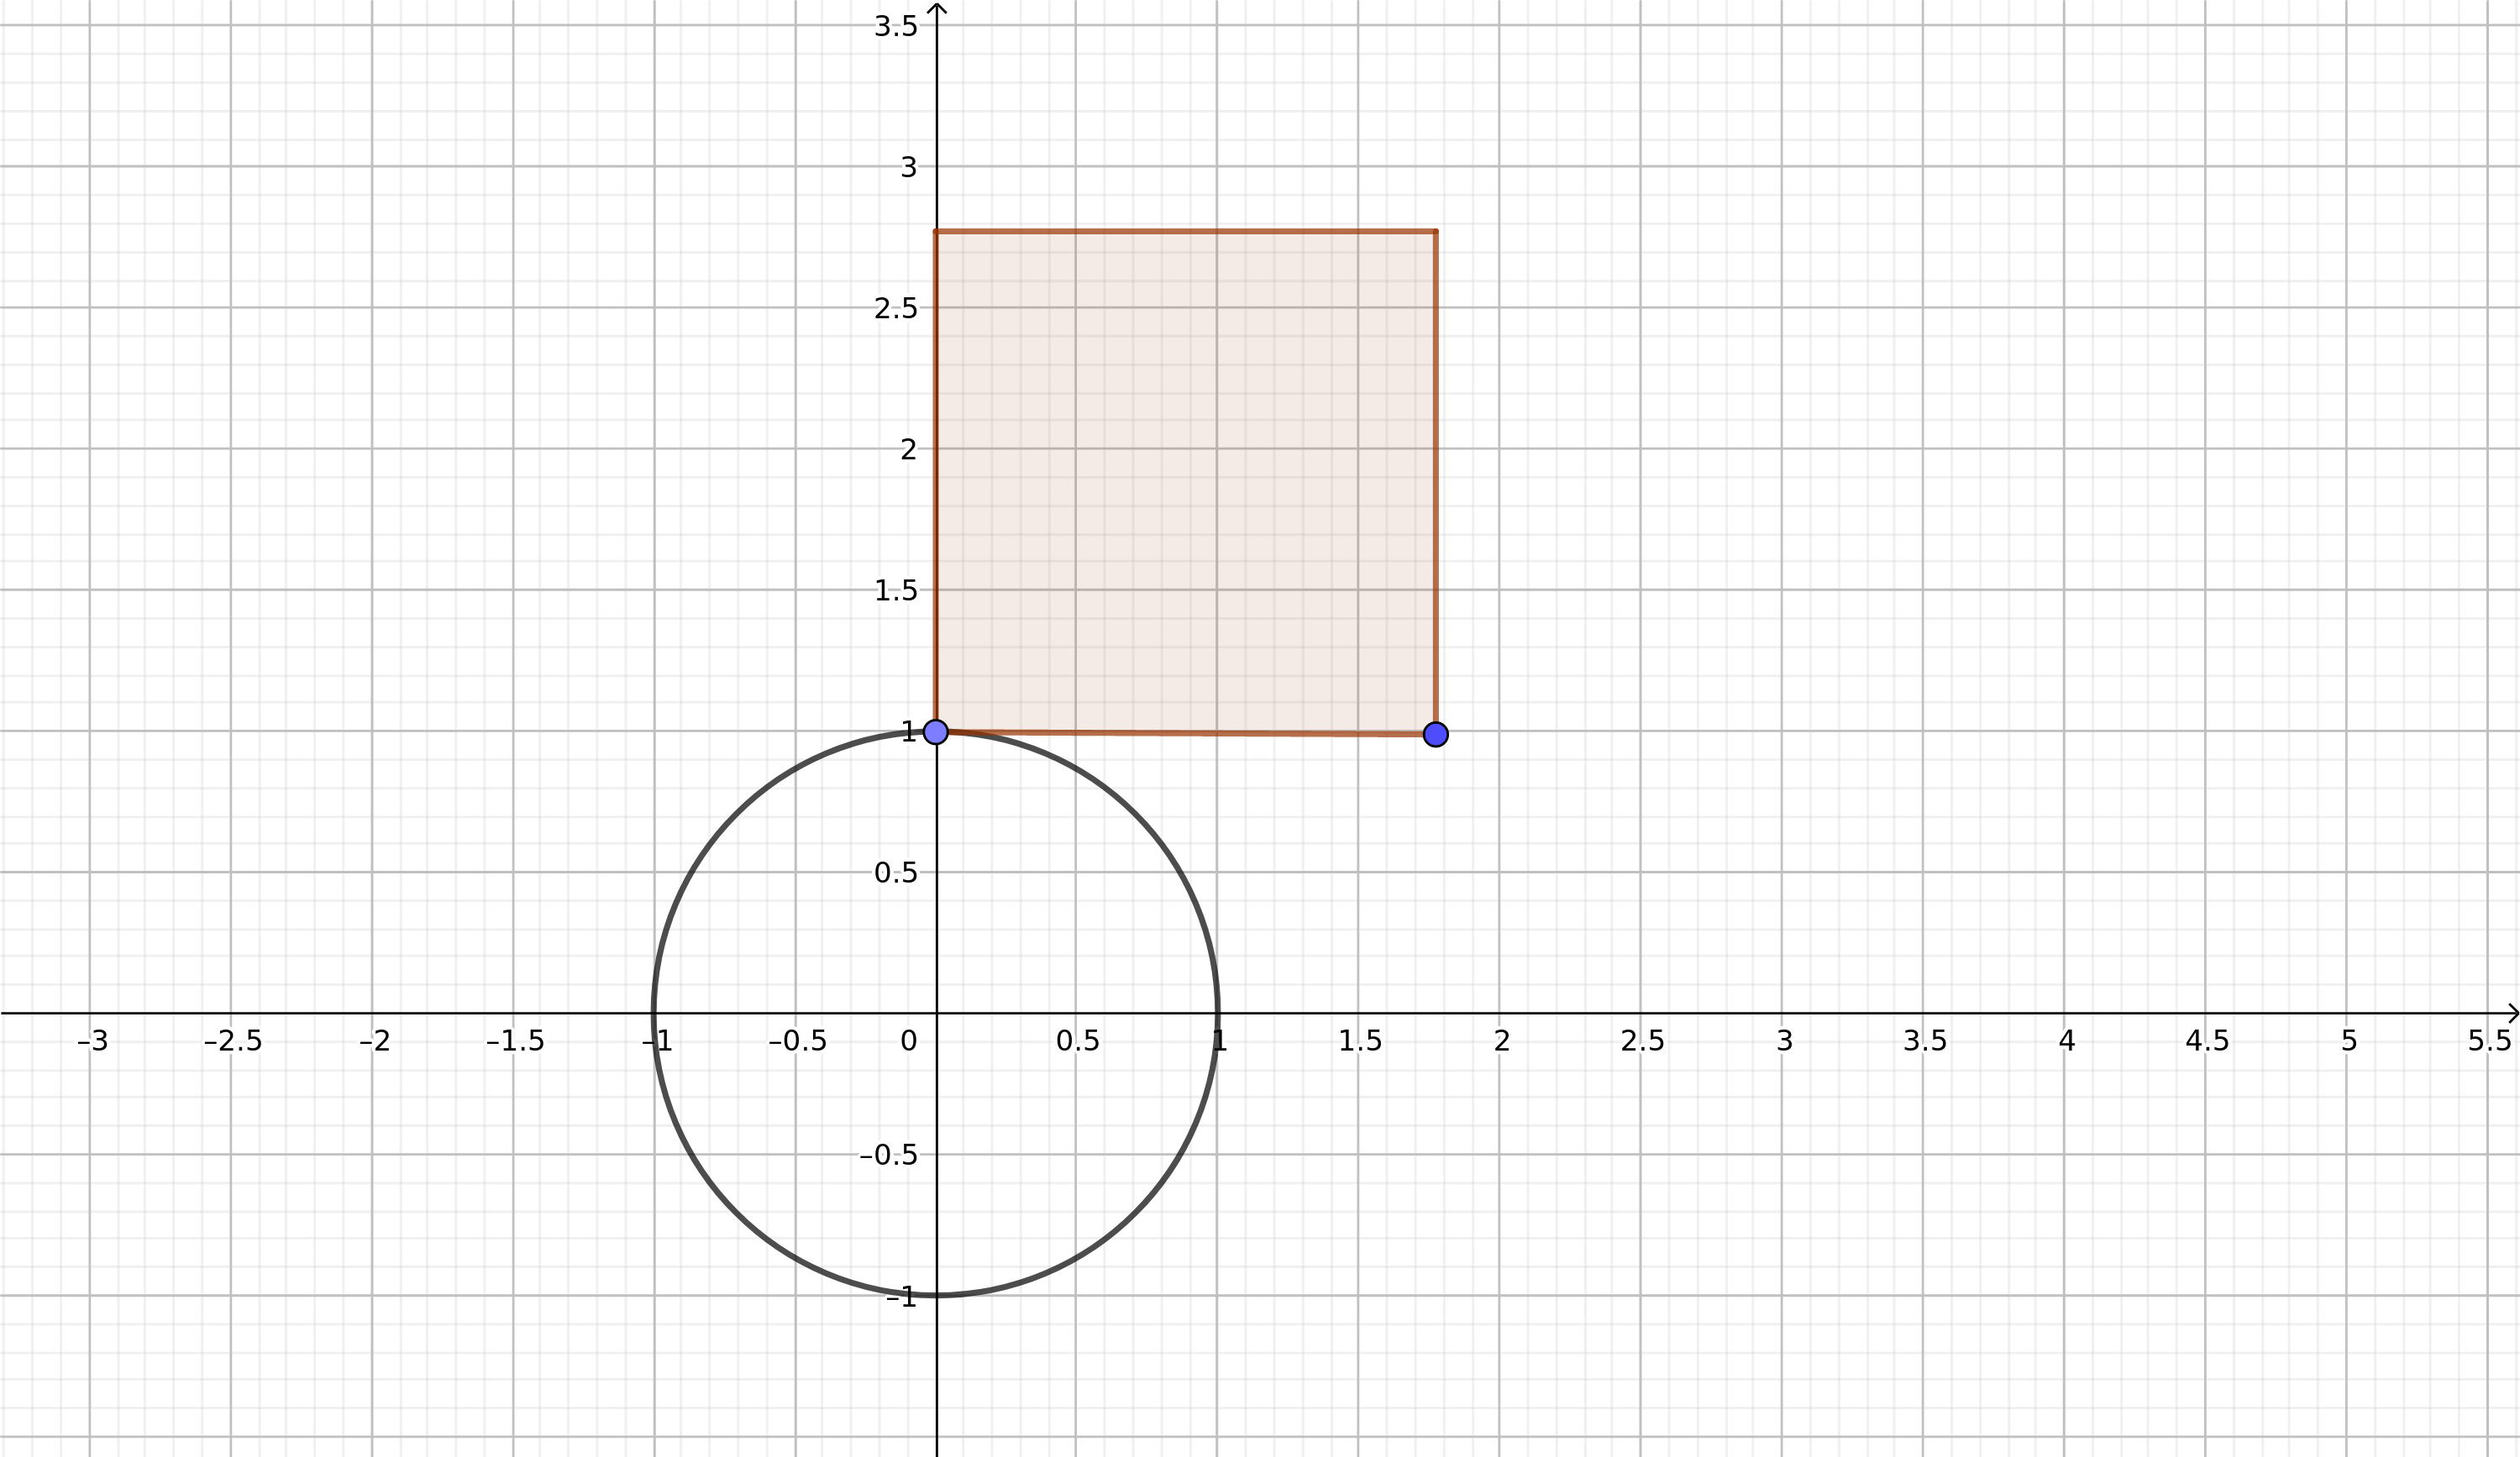
\includegraphics[width=0.6\textwidth]{Negativ-QuadraturDesKreises1.png}
	\caption{Quadratur des Kreises: konstruiere mit Zirkel und Lineal ein Quadrat mit dem gleichen Flächeninhalt von einem gegebenem Kreis.}
\end{figure}

Betrachte das Problem der ''Triangularisierung'' des Kreises. Dieses Problem bezeichnen wir mit \(D_{\bigcirc}\) und definieren wie folgt: Gegeben ein Kreis, konstruiere mit Zirkel und Lineal in endlich viele Schritten ein rechtwinkliges gleichschenkliges Dreieck, so dass das Dreieck und der Kreis den gleichen Flächeninhalt haben.
\begin{figure}[H]
	\centering
	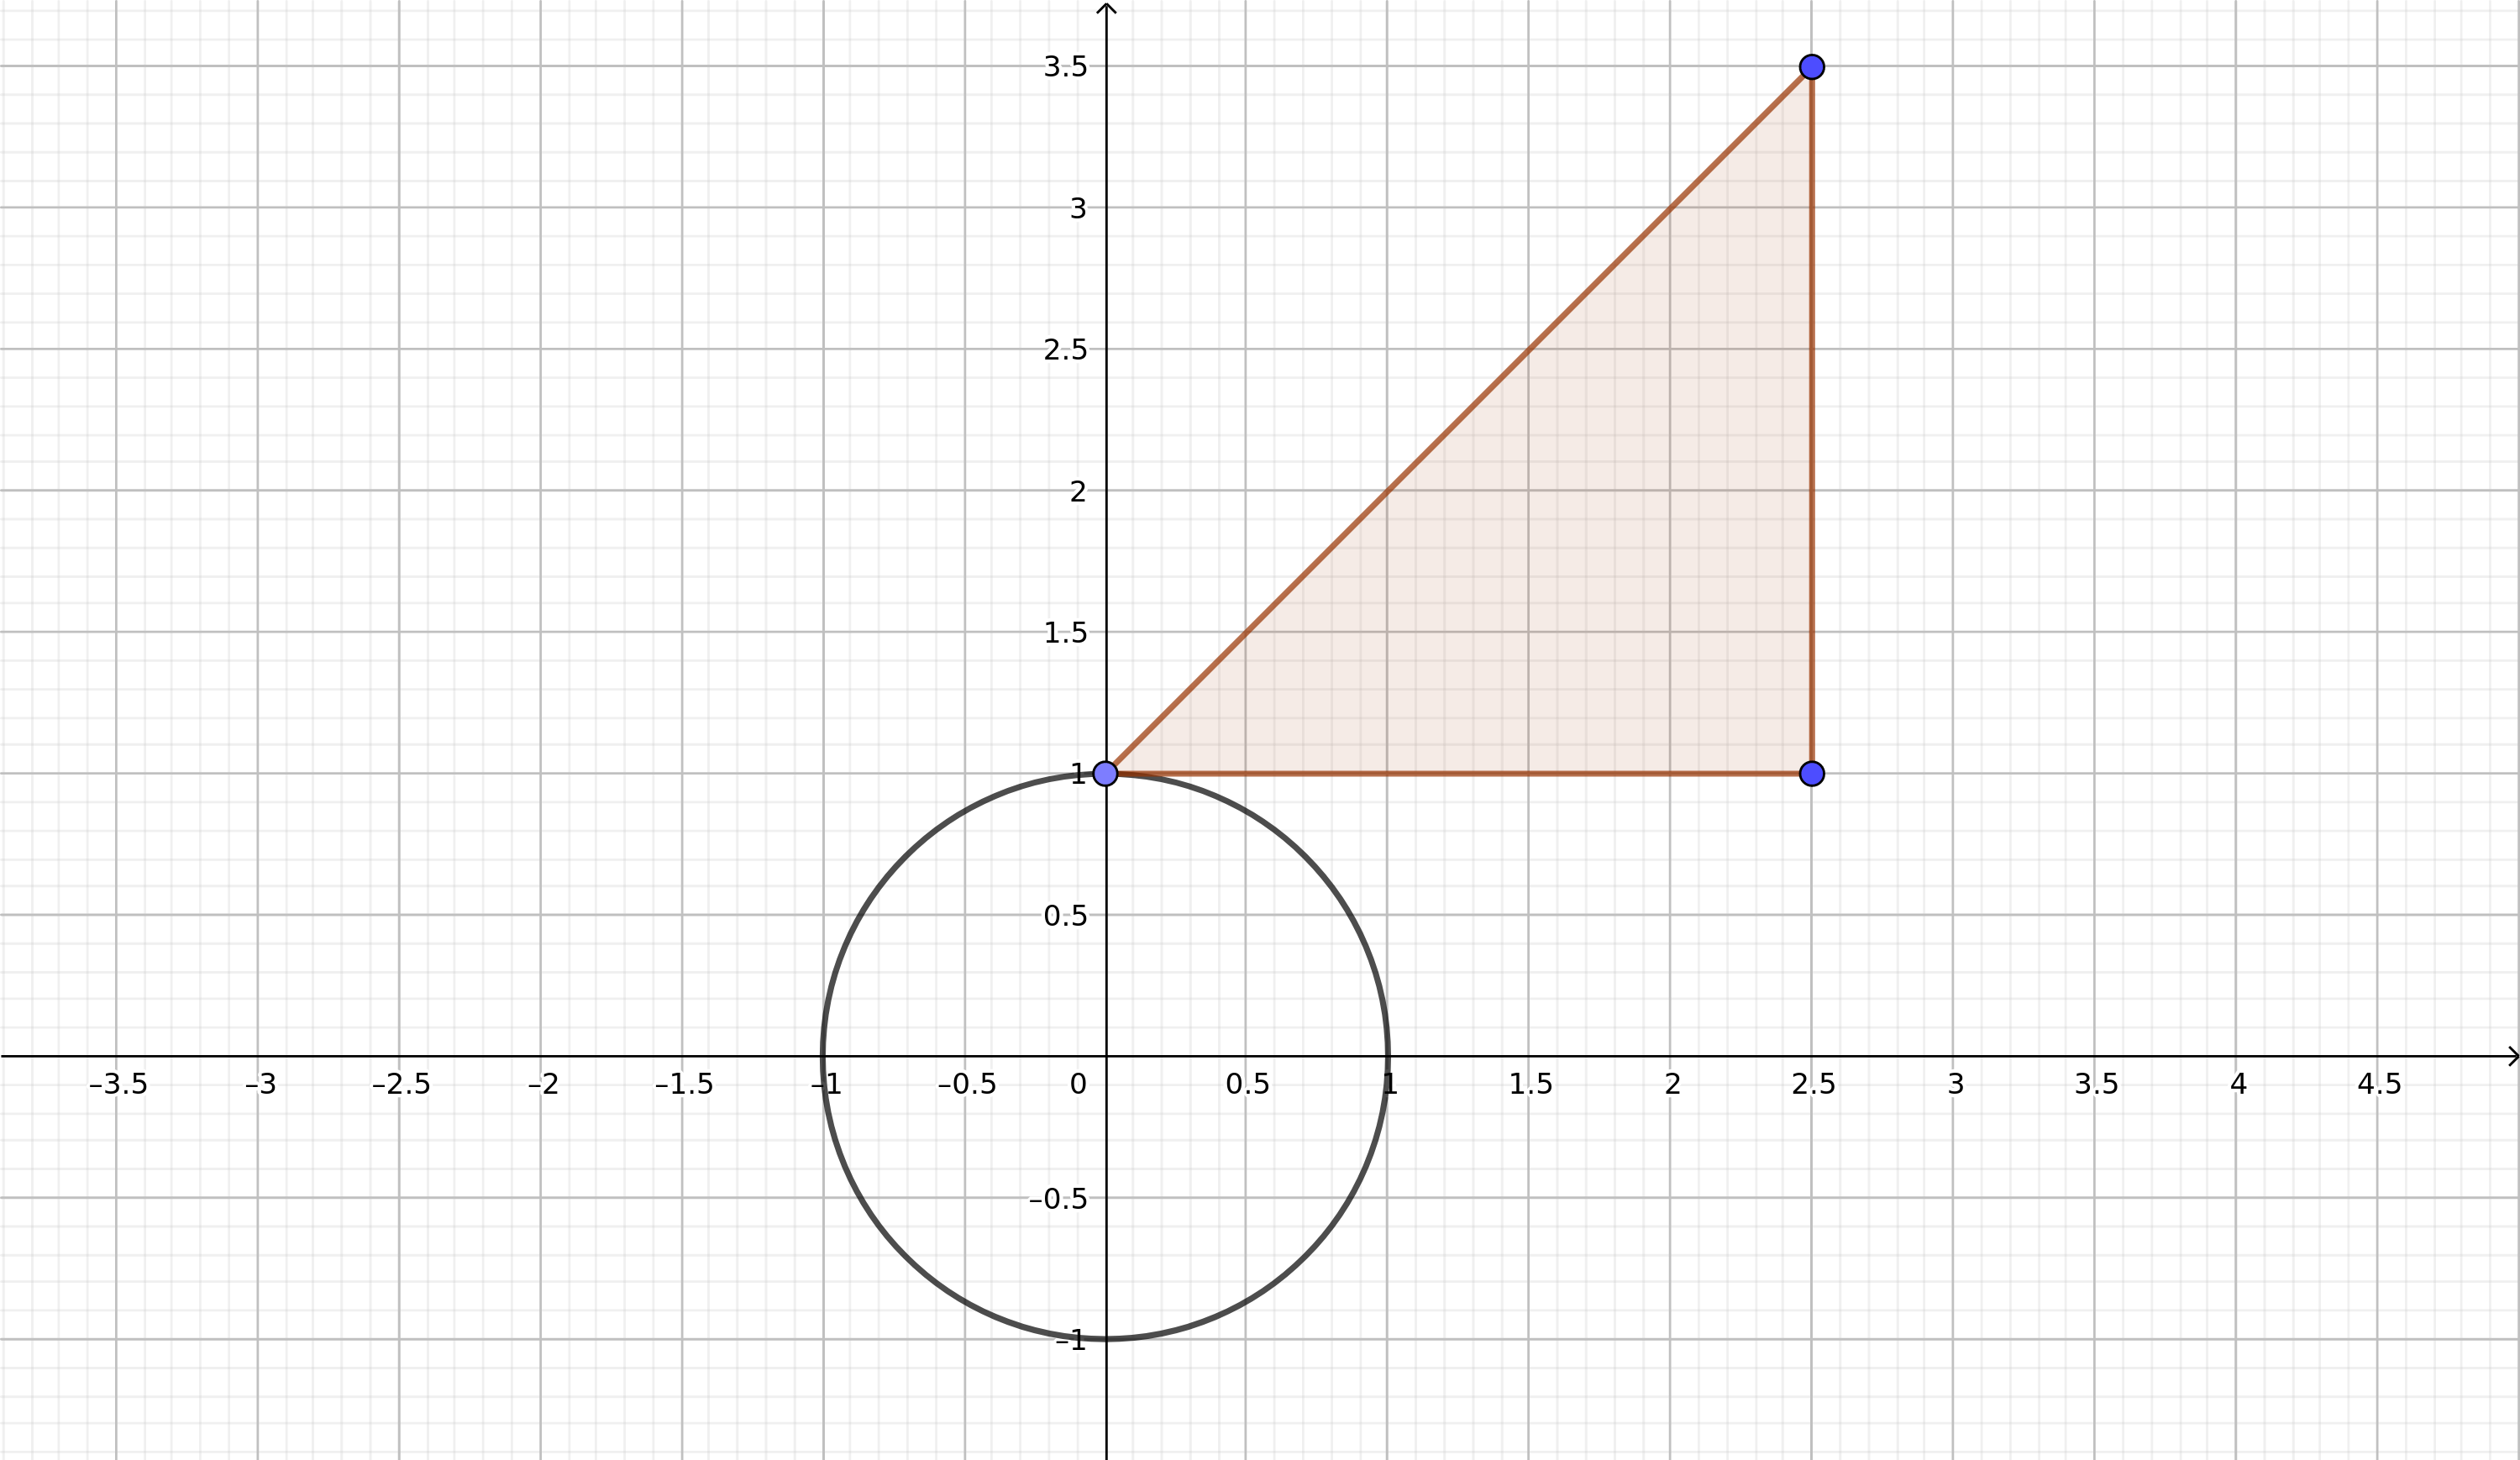
\includegraphics[width=0.6\textwidth]{Negativ-TriangulaturDesKreises1.png}
	\caption{''Triangularisierung'' des Kreises: konstruiere mit Zirkel und Lineal ein rechtwinkliges gleichschenkliges Dreieck mit dem gleichen Flächeninhalt von einem gegebenem Kreis.}
\end{figure}
Beweise mittels Reduktion, dass kein ZL-Algorithmus zur ''Triangularisierung'' des Kreises existiert.
\end{problem}

%------------------------------------------------

\subsection*{Musterlösung}

Wir wissen, dass es keinen ZL-Algorithmus für \(Q_{\bigcirc}\) gibt und möchten diese Tatsache benutzen, um zu zeigen, dass es keinen ZL-Algorithmus für \(D_{\bigcirc}\) gibt.

Wir nutzen dabei die Methode des indirekten Beweises: Wir nehmen das Gegenteil von dem an, was wir beweisen möchten, und folgern daraus etwas Falsches. Das impliziert, dass unsere Annahme falsch sein muss, und somit haben wir genau das bewiesen, was wir wirklich beweisen wollten.

In diesem Fall nehmen wir also an, dass wir einen ZL-Algorithmus für \(D_{\bigcirc}\) haben und konstruieren daraus einen ZL-Algorithmus für \(Q_{\bigcirc}\). Da es keinen solchen Algorithmus gibt, muss unsere Annahme falsch sein.

Wir reduzieren also \(Q_{\bigcirc}\) auf \(D_{\bigcirc}\) und zeigen \(Q_{\bigcirc} \leq_{Alg} D_{\bigcirc}\). Aus \(Q_{\bigcirc} \leq_{Alg} D_{\bigcirc}\) und \(Q_{\bigcirc}\) unlösbar folgern wir, dass \(D_{\bigcirc}\) auch unlösbar sein muss.

Sei \(A_d\) ein ZL-Algorithmus, welcher \(D_{\bigcirc}\) löst. Diesen Algorithmus benutzen wir, um einen ZL-Algorithmus \(A_q\) für \(Q_{\bigcirc}\) zu konstruieren. Dafür müssen wir mit Zirkel und Lineal in endlich vielen Schritten ein Quadrat konstruieren, welches den gleichen Flächeninhalt von einem gegebenem rechtwinkligem gleichschenkligem Dreieck hat.

Möglich wäre folgende Abfolge:
\begin{figure}[H]
	\centering
	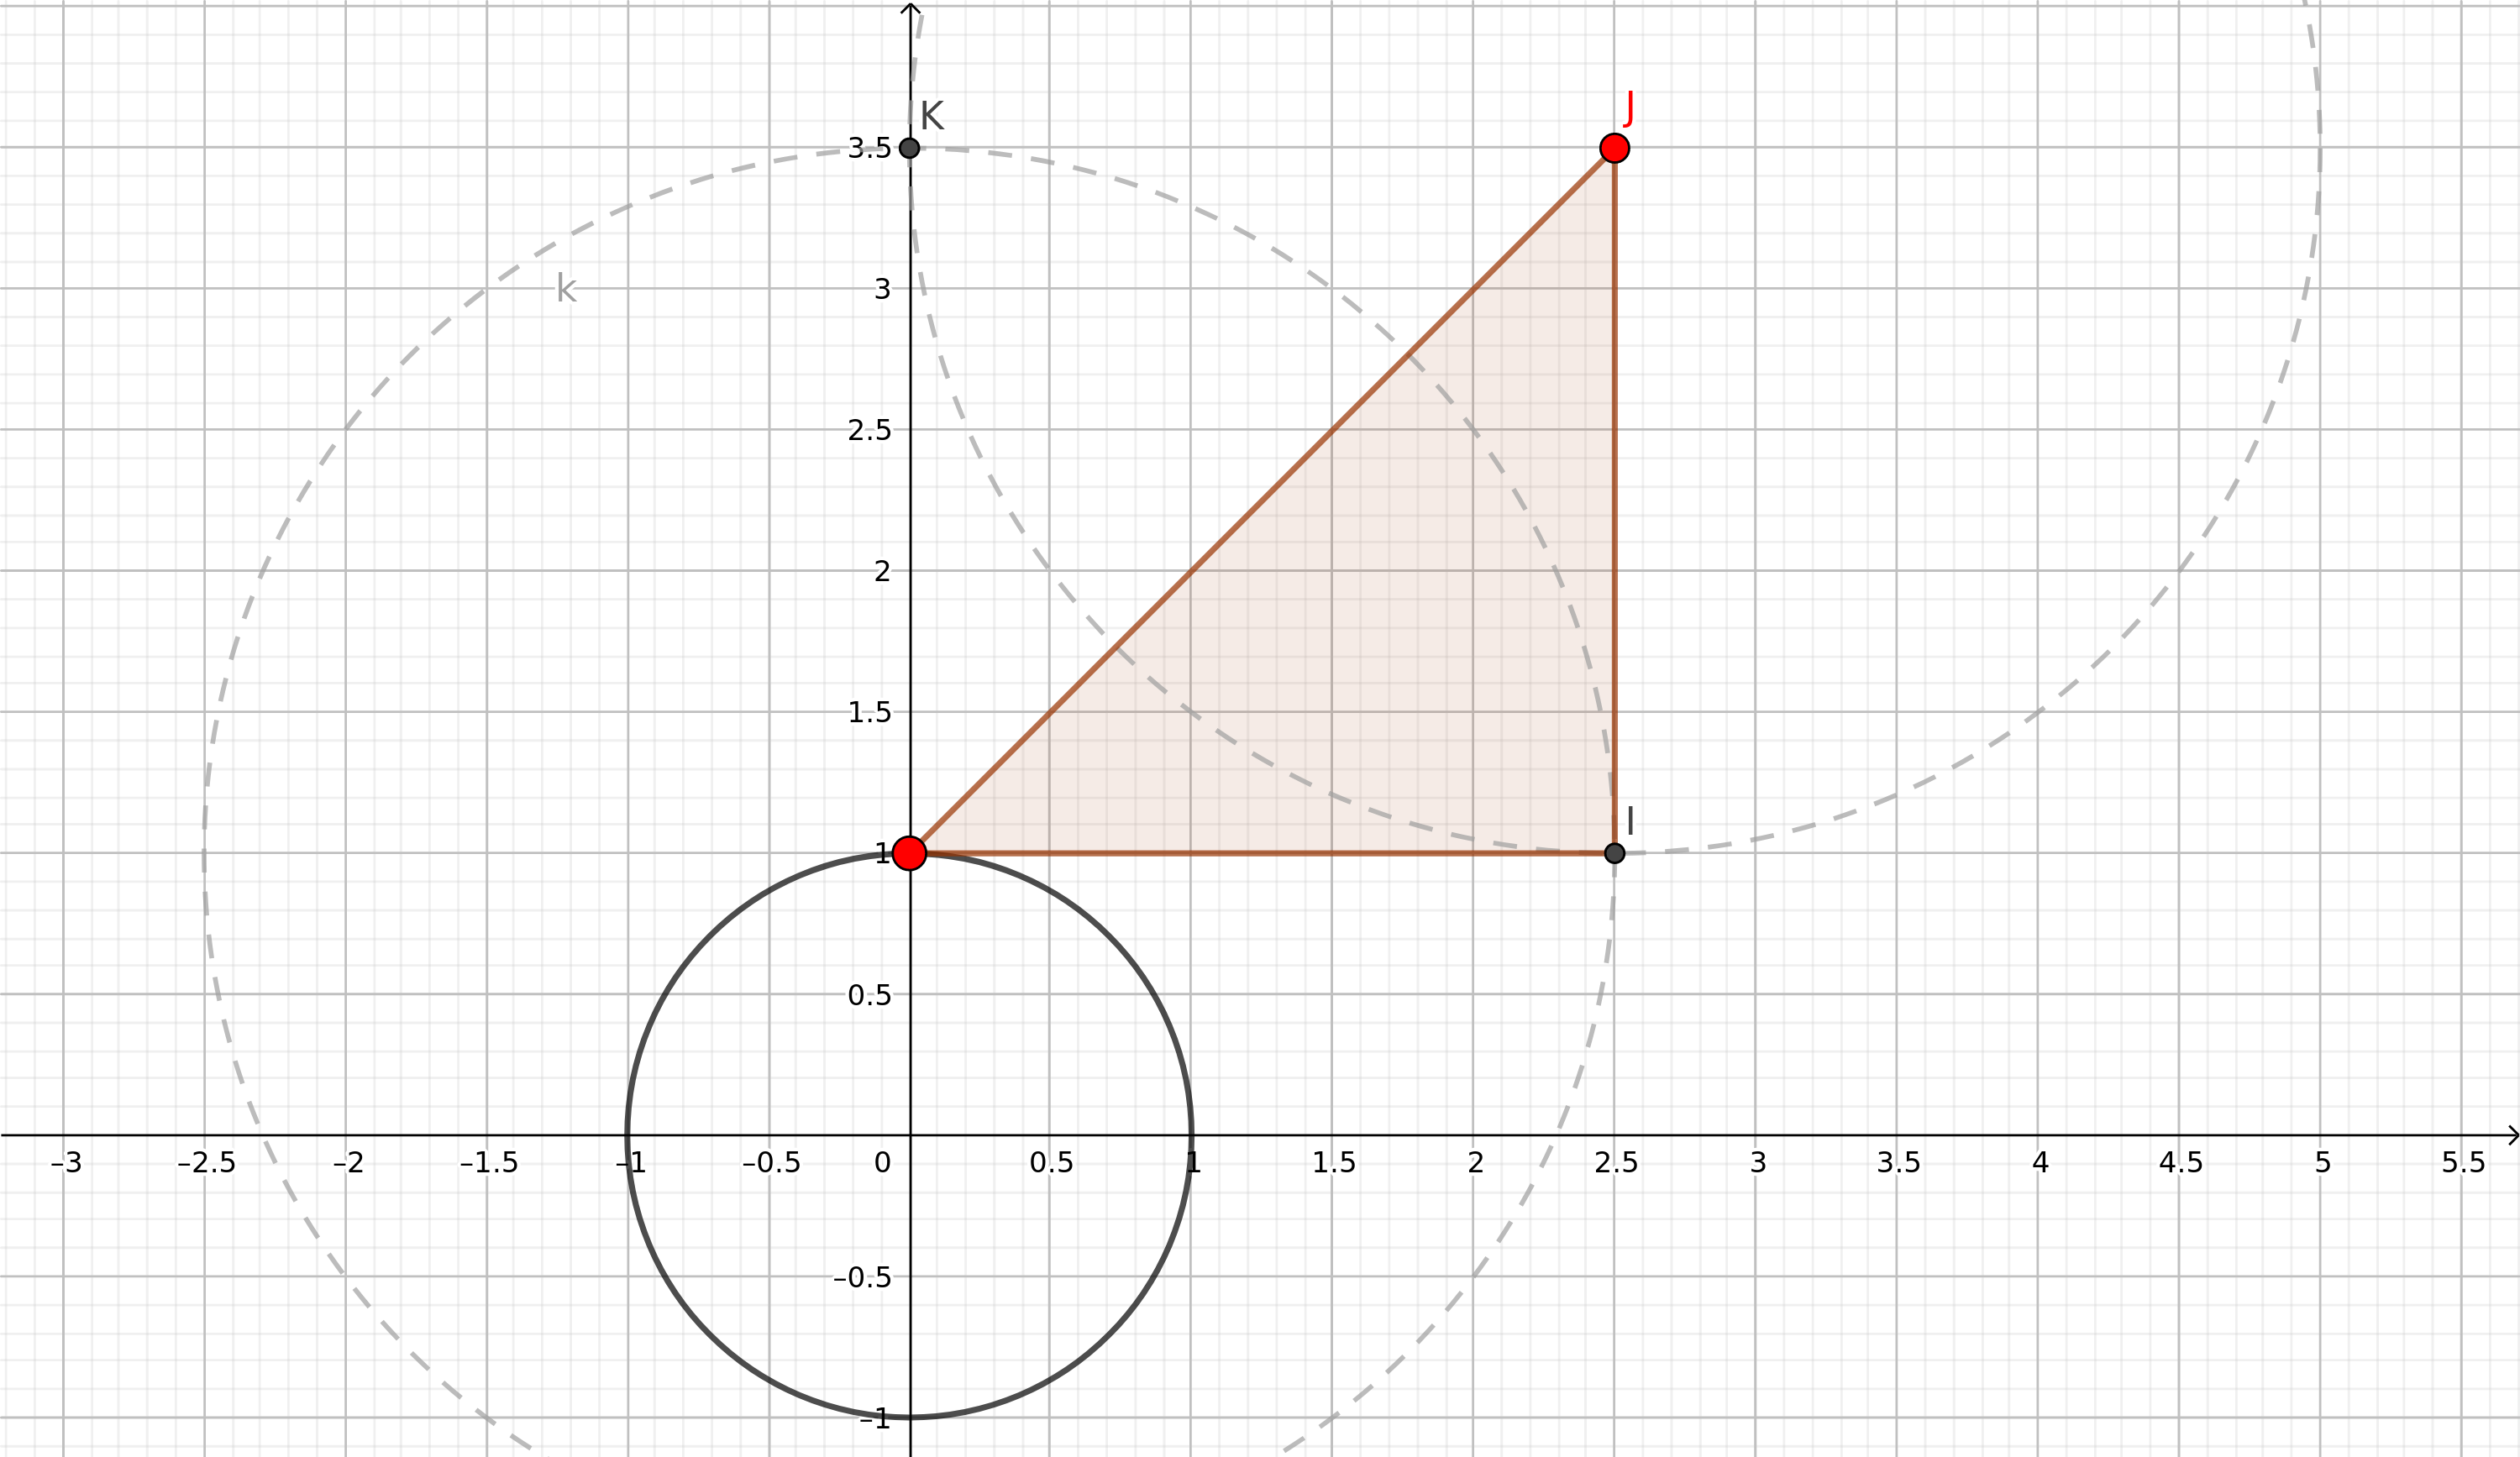
\includegraphics[width=0.6\textwidth]{Negativ-TriangulaturDesKreises2.png}
\end{figure}
\begin{figure}[H]
	\centering
	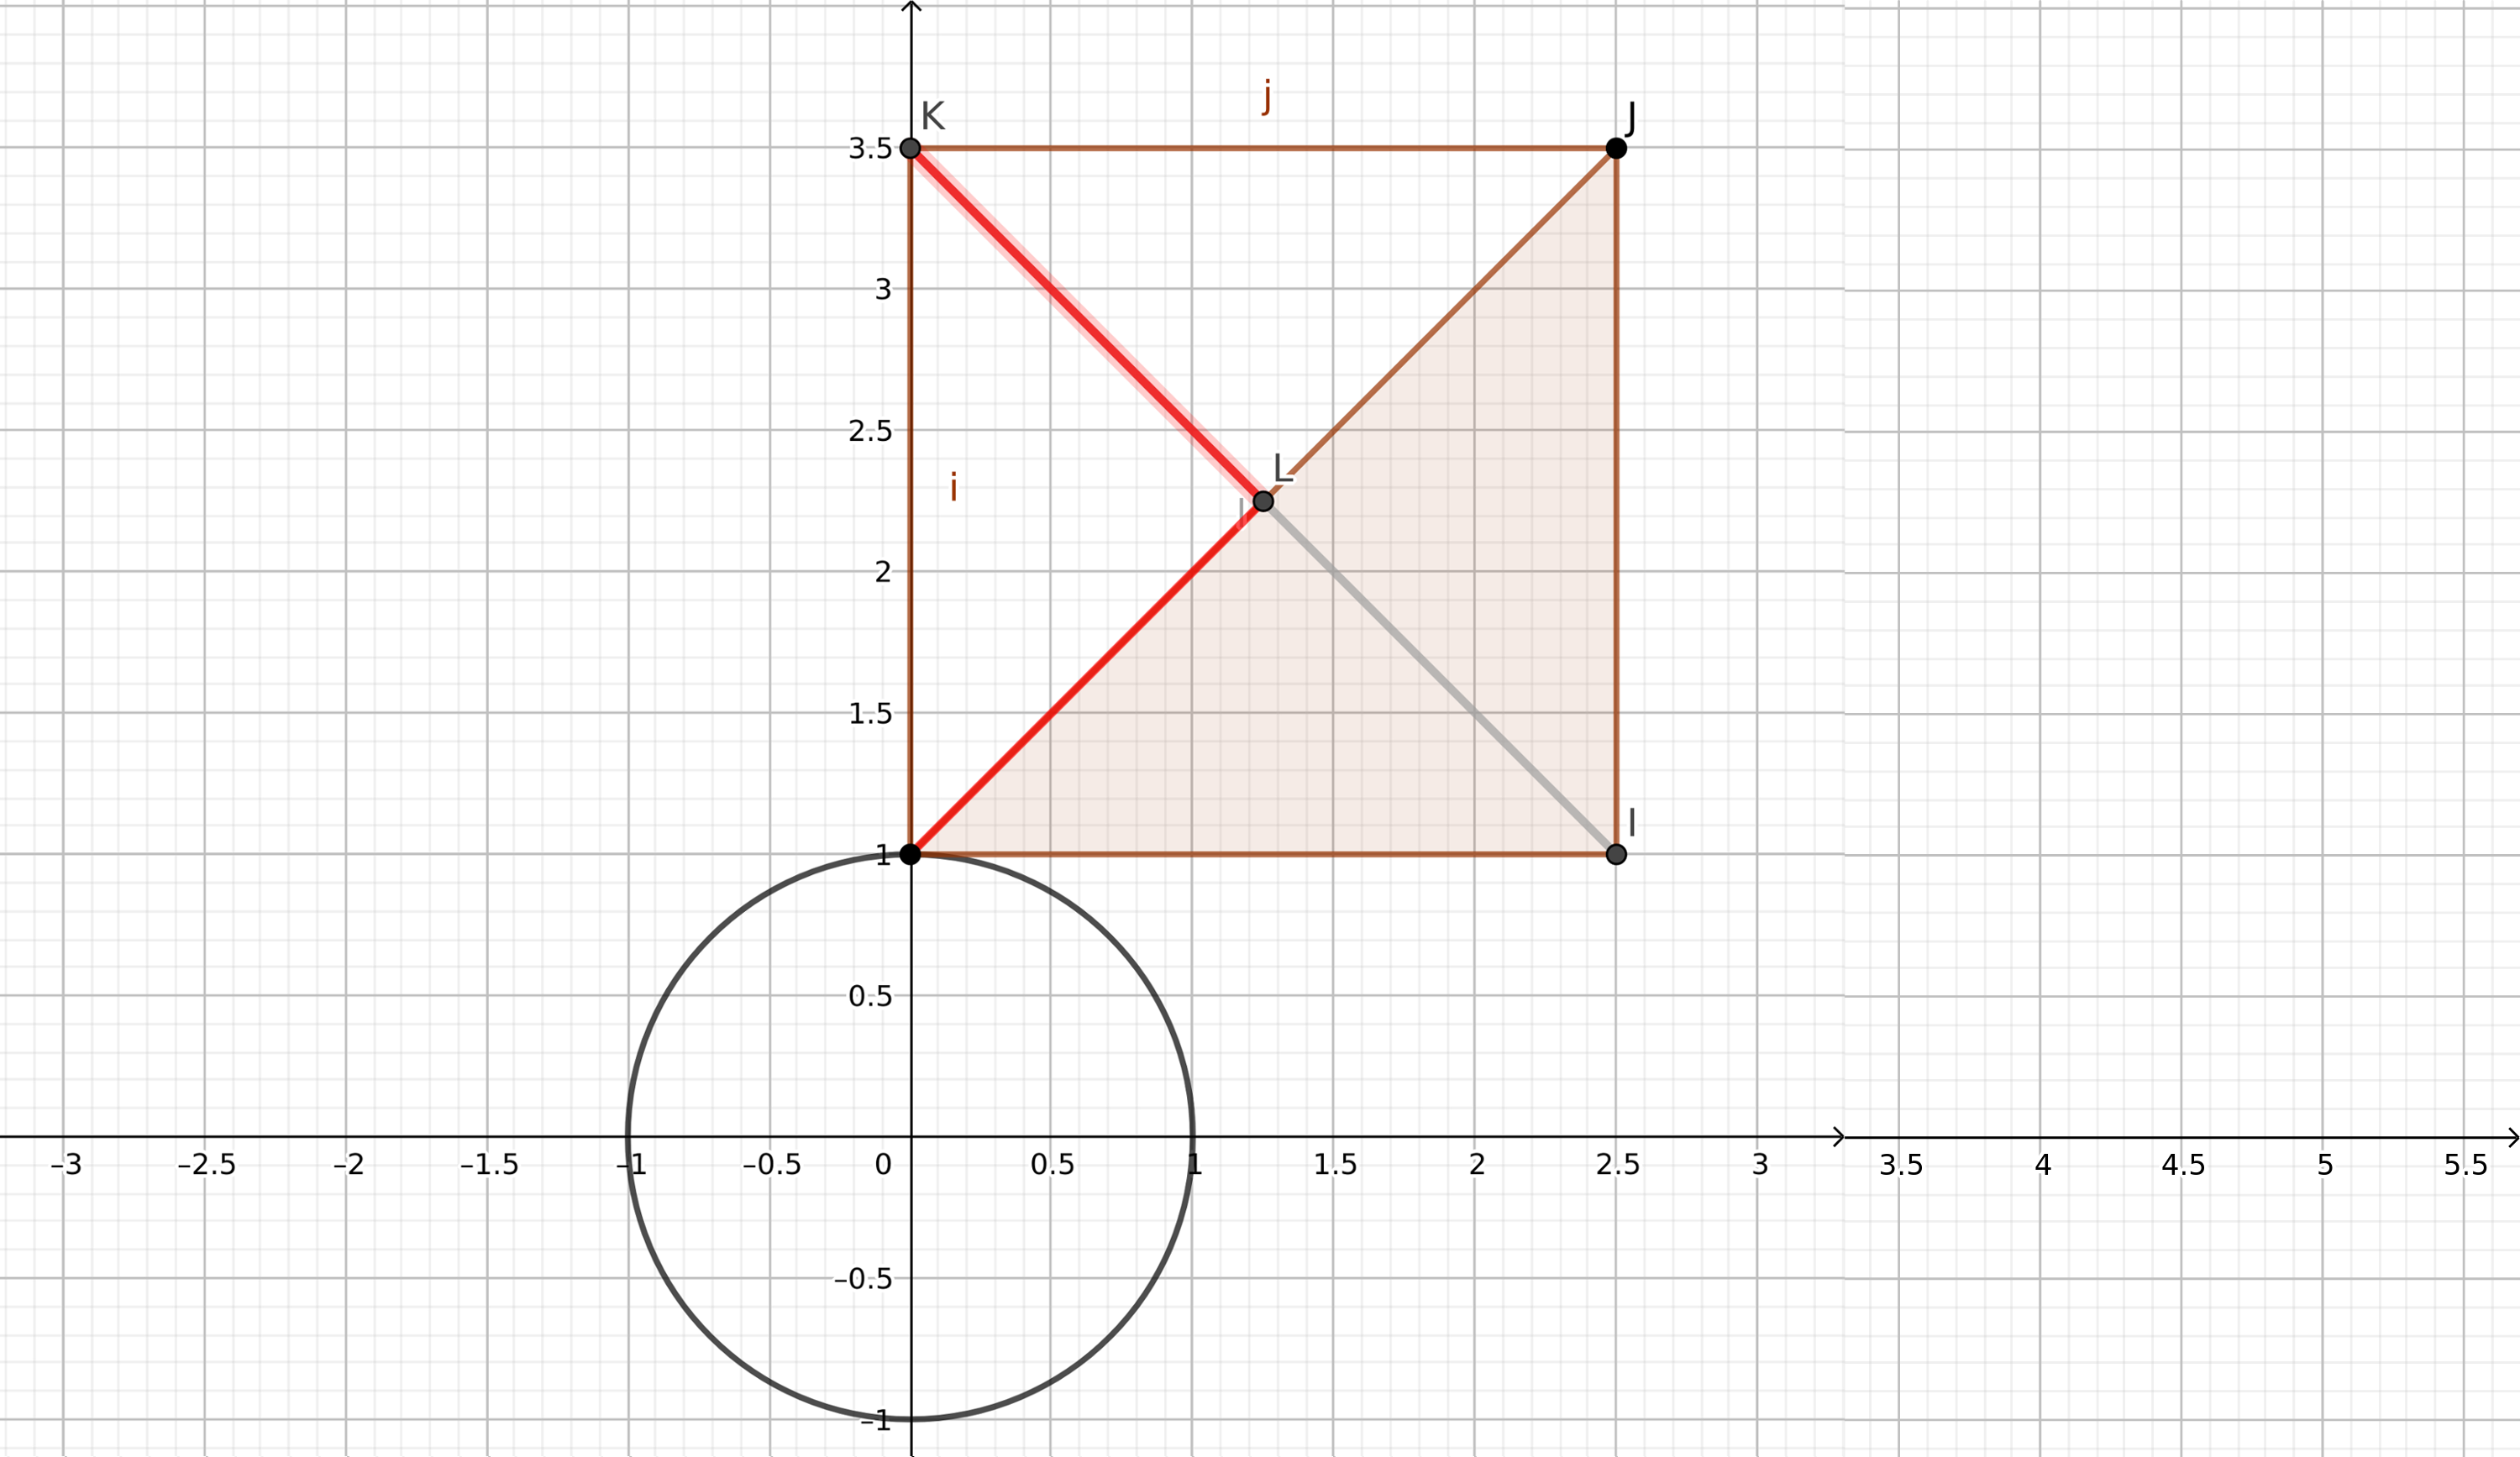
\includegraphics[width=0.6\textwidth]{Negativ-TriangulaturDesKreises5.png}
\end{figure}\begin{figure}[H]
	\centering
	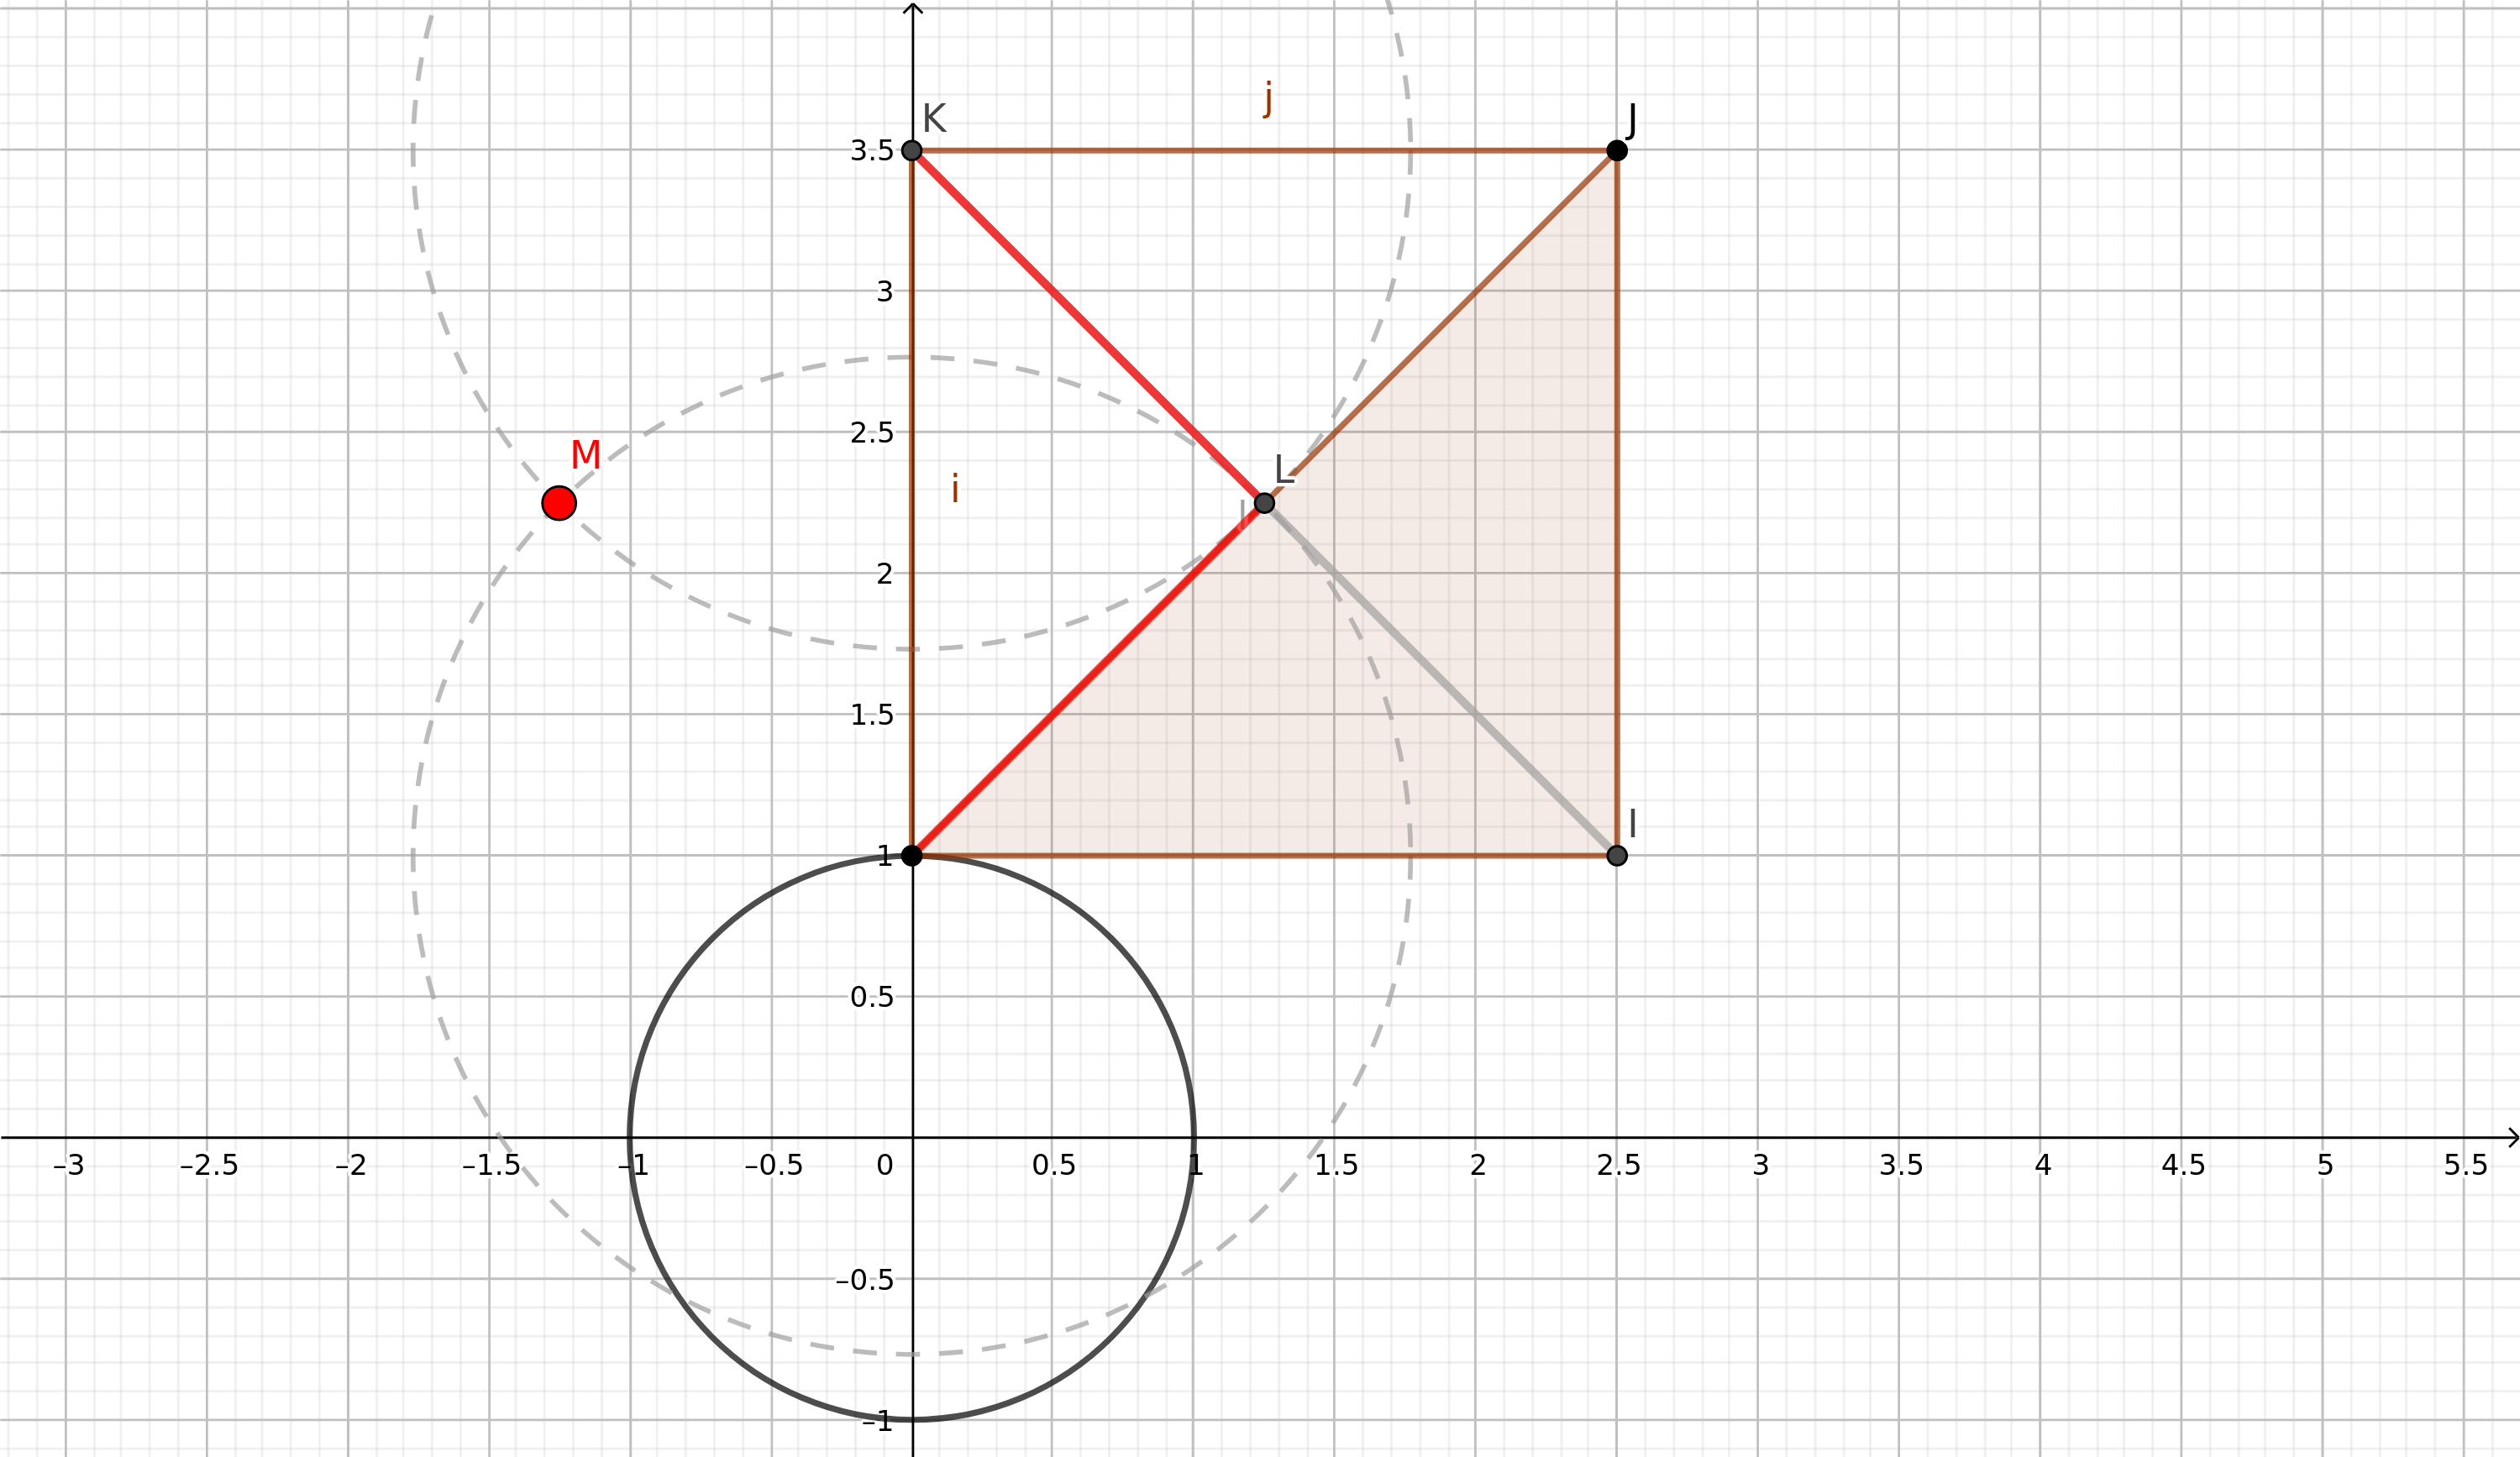
\includegraphics[width=0.6\textwidth]{Negativ-TriangulaturDesKreises6.png}
\end{figure}\begin{figure}[H]
	\centering
	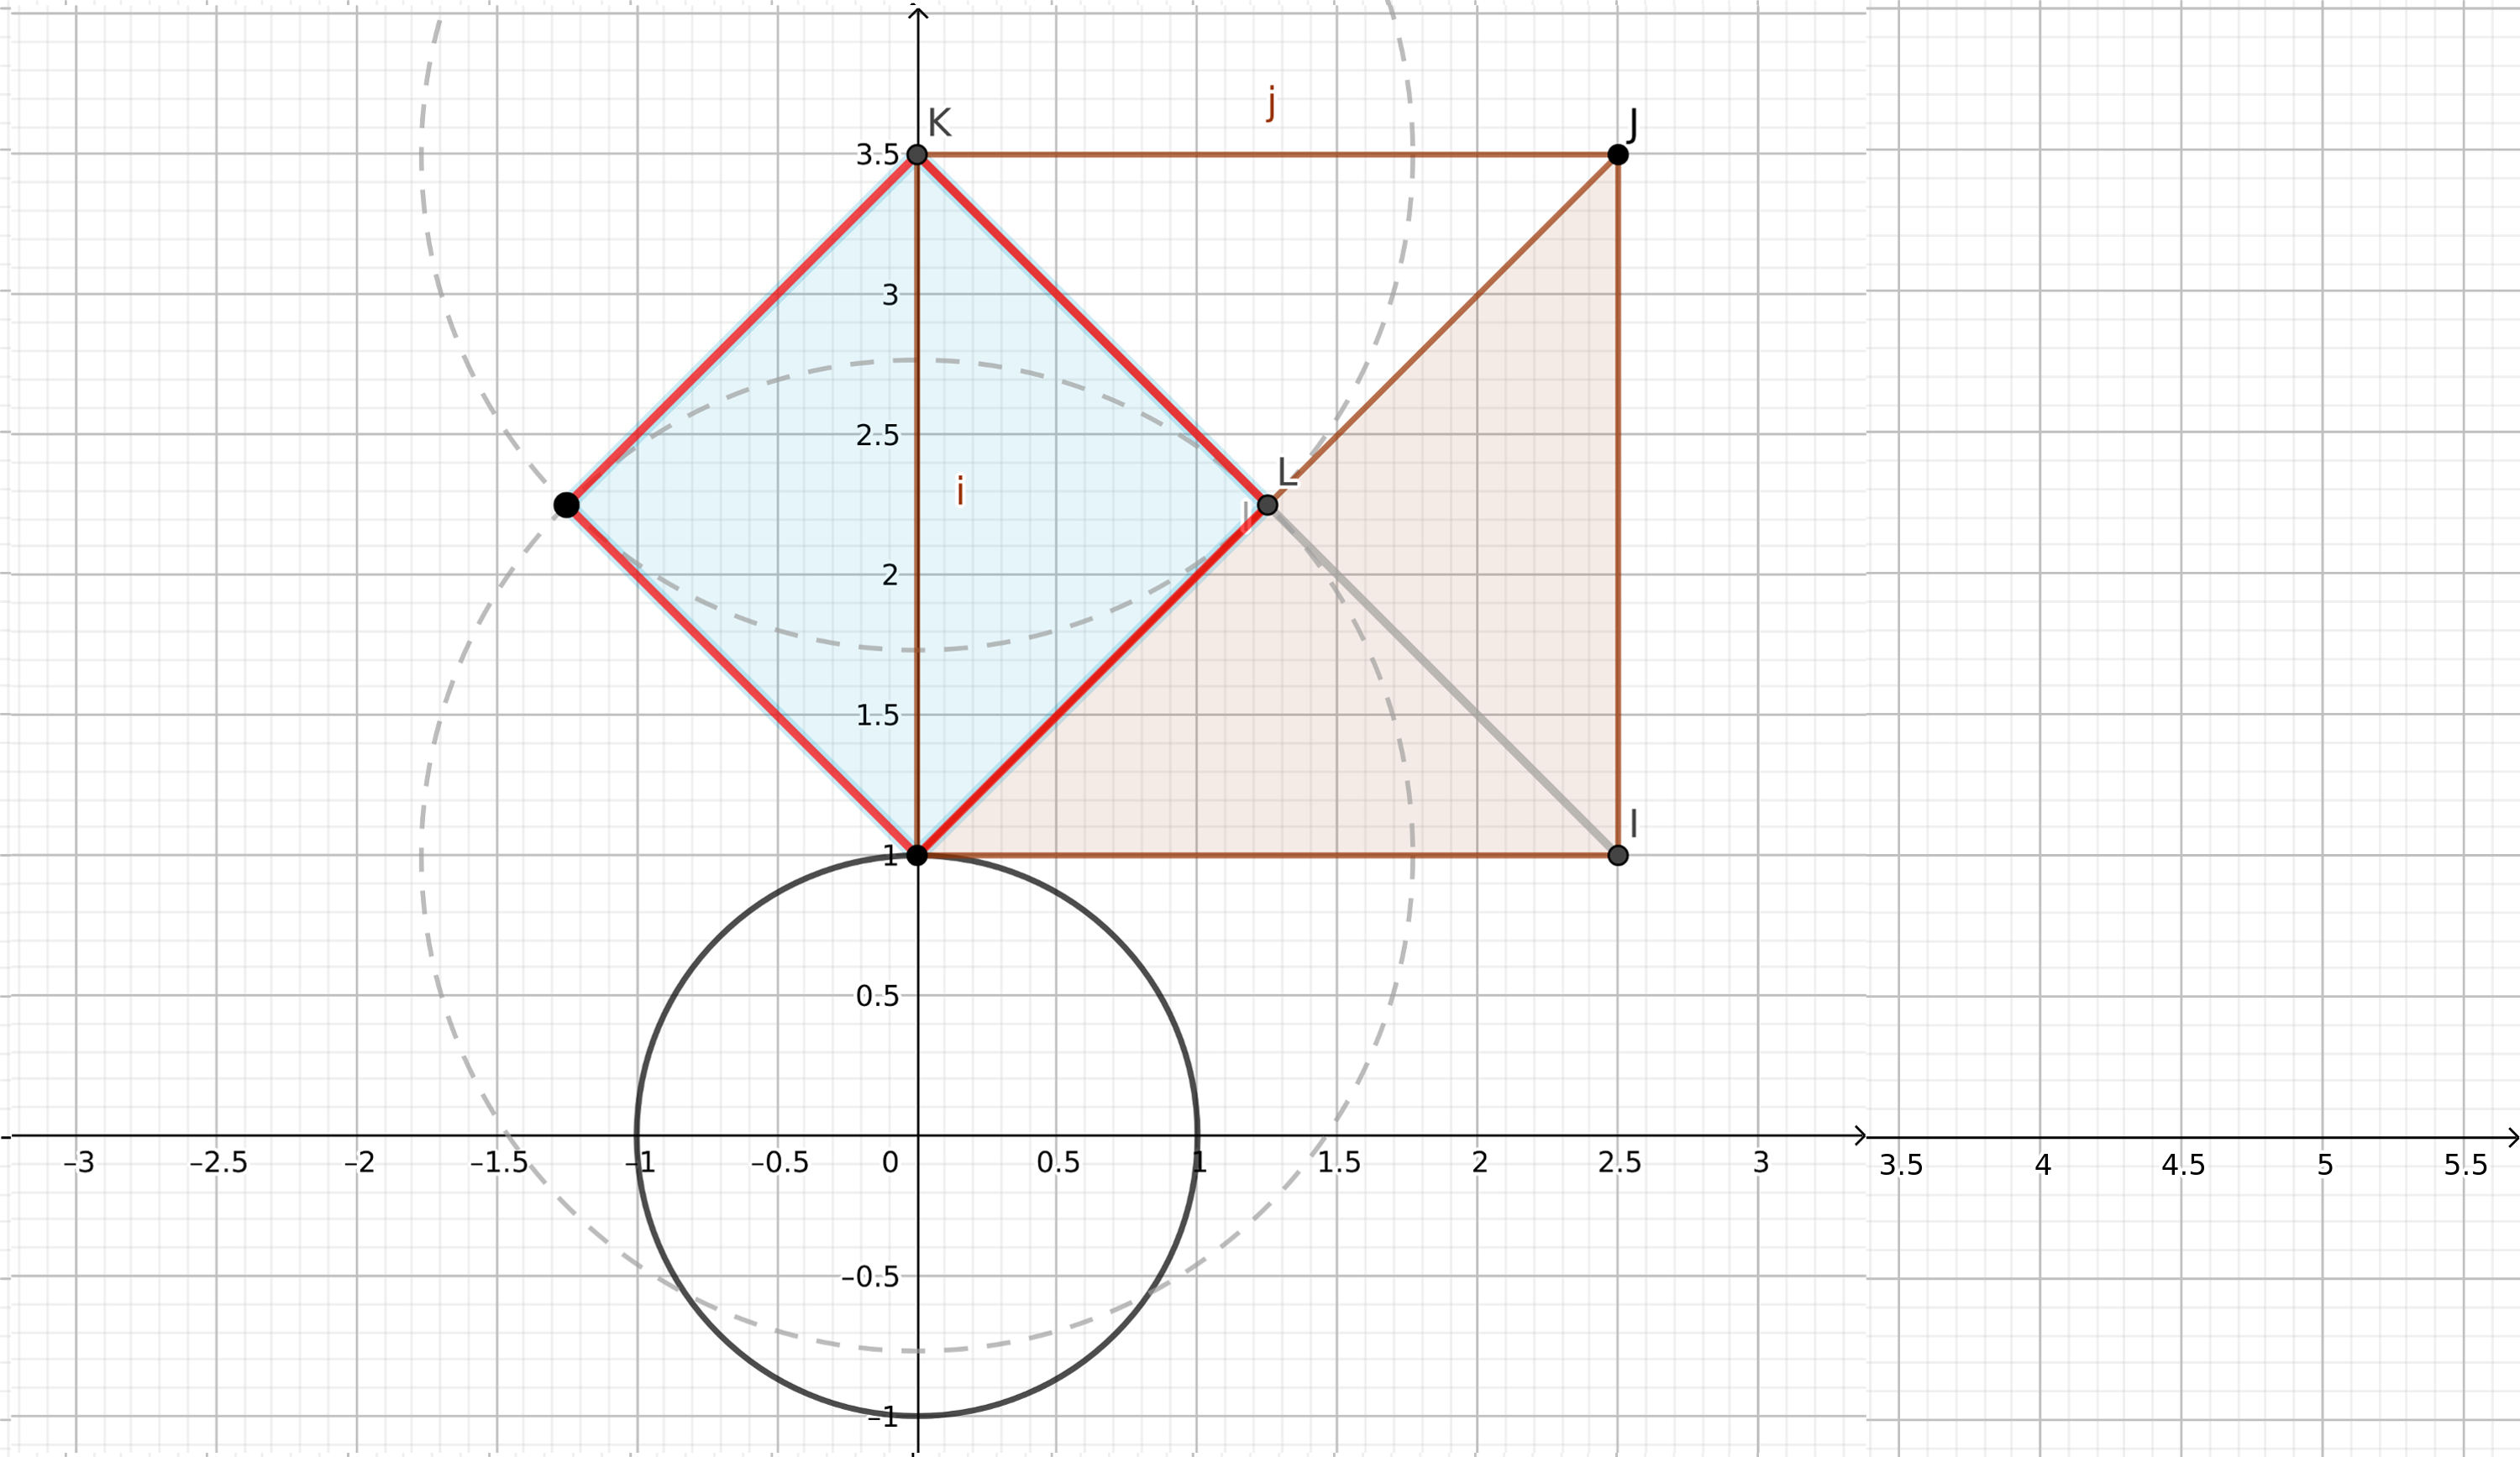
\includegraphics[width=0.6\textwidth]{Negativ-TriangulaturDesKreises7.png}
\end{figure}

Somit haben wir den ZL-Algorithmus \(A_q\) aus \(A_d\) konstruiert, welcher die Quadratur der Kreises findet. Da ein solcher Algorithmus nicht existiert, haben wir bewiesen, dass \(A_d\) nicht existieren kann.
\begin{figure}[H]
	\centering
	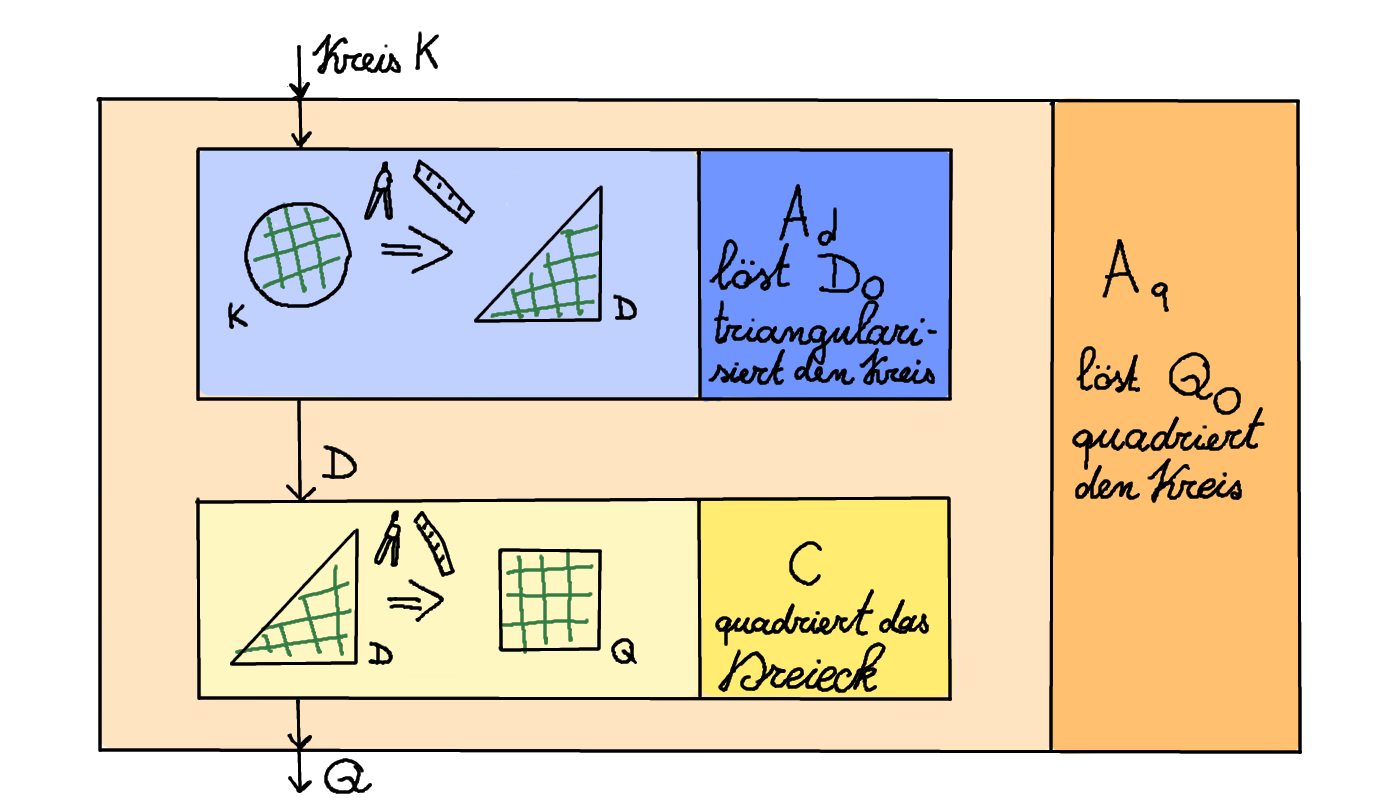
\includegraphics[width=\textwidth]{Negativ.png}
	\caption{Reduktion von \(Q_{\bigcirc}\) auf \(D_{\bigcirc}\).}
\end{figure}


\end{document}
